\chapter{Unifying Logic} \label{uni}
% \setlength{\epigraphrule}{0pt}
% \setlength{\epigraphwidth}{0.75\textwidth}
% %\epigraph{\textit{Er ist ein Mathematiker und also hartnäckig.}}{Johann Wolfgang von Goethe}
% \epigraph{\textit{[Socrates] ita disputat, ut [...] nihil se scire dicat nisi id ipsum, eoque praestare ceteris, quod illi quae nesciant scire se putent, ipse se nihil scire id unum sciat.}}{Cicero, Academica 1,16}

In this chapter we discuss the idea of a unifying logic for the Semantic Web. The term itself stems form the so-called \emph{Semantic Web Stack}.
This schema represents the envisioned architecture for the Semantic Web and the unifying logic is one of its pieces.
Therefore we start with a discussion of that stack in general to then focus on the parts relevant for this thesis. These considerations then lead to the research questions.


\section{The architecture of the Semantic Web}
 To concretely realise the dream of a machine understandable Web as it was envisioned by Tim Berners-Lee et al. \cite{SemanticWeb}, 
an architecture has been proposed, the  
 \emph{Semantic Web Stack} (aka \emph{Semantic Web Layer Cake}).
This stack provides a structural overview of the different concepts, technologies and standards needed for the Semantic Web to become reality. 
Its shape has changed over the years \cite{Gerber2} due to the progress made---several languages such as \rdf \cite{rdf} and SPARQL \cite{sparql} have been standardised---but also 
as a consequence of controversial discussion \cite{twotowers,rearch}. 
Knowing that this version can---and most probably will---evolve and change in the coming years, 
we focus %current 
%version from wikipedia, which is a slight modification of 
on the latest official 
variant %\footnote{Available at: \url{https://www.w3.org/2007/03/layerCake.svg}.} 
 and discuss its different parts. This variant is displayed in Figure~\ref{fig:stack}.\footnote{Colours and shapes are changed in this version to make it fit better into this book. 
The original picture is available at: 
\url{https://www.w3.org/2007/03/layerCake.svg}.
A newer (unofficial) version is for example provided by Hogan \cite{hogan}.} 
\begin{figure}[!ht]
	\centering
	%\begin{adjustwidth}{-\marginnotewidth}{}%
	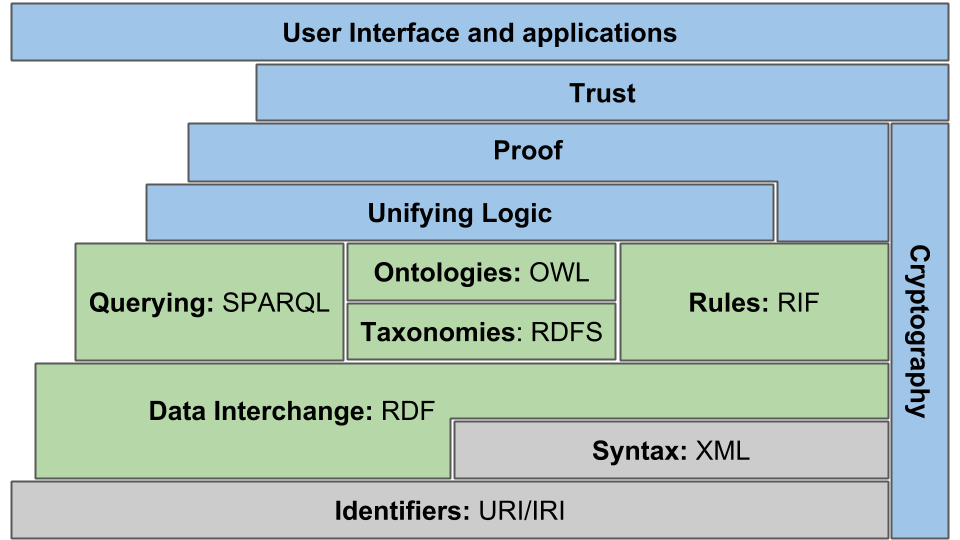
\includegraphics[width=0.8\textwidth]{stack6}
	%\end{adjustwidth}
	\caption[Semantic Web Stack]{Semantic Web Stack.}
	\label{fig:stack}
\end{figure}
%\footnotetext{Source: \url{https://en.wikipedia.org/wiki/Semantic_Web_Stack}}
Each layer placed on top of other layers  depends on  these other layers but not on those above them. Neighbouring layers can, but not necessarily have to make use of each other. 
We go from the bottom of the stack to its top to explain all its elements:

\begin{description}
%  \item[Character Set] To be compatible with the current Web and its applications, but also with textual documents in all languages in general,
%  the Semantic Web relies on Unicode.
 \item[Identifiers] The Semantic Web is a global network which relies on interoperability. In such a big setting, it is crucial that the names of individuals and concepts are unique.
 For their representation Uniform Resource Identifiers (\uris) and Internationalized Resource Identifiers (\iri{}s) are used.  
 \item[Syntax] There are several syntax formats frequently used in the Semantic Web. Standards of the World Wide Web are employed---such as XML or JSON---but also formats 
 only created for the Semantic Web such as for example the Terse RDF Triple Language (Turtle). 
%  The fact that the Semantic Web stack only mentions XML and omits 
%  other notations which are also used
%  is often 
%  a point of criticism.\footnote{See for example the discussion at: \url{https://lists.w3.org/Archives/Public/semantic-web/2016Feb/0121.html}.} 
 \item[Data Interchange]
In order to exchange data it must be agreed on  a common structure to express knowledge. This 
structure should not be too complex for a machine to parse but still 
powerful enough to make simple statements and connections. 
In the Semantic Web the Resource Description Framework (\rdf) was developed with 
that goal in mind. Knowledge is expressed using simple triples consisting of subject,
predicate and object. By using unique names (\iri{}s and \uris) connections between different triples are made. 
Ideally, one resulting graph then forms the Semantic Web.
 \item[Taxonomies] For the simple classification of objects and properties the Semantic Web uses the standard \rdf Schema (\rdf{}S). \rdf{}S extends the basic representation format 
 \rdf by several predicates with a predefined meaning such as for example \texttt{rdfs:subclassOf} to denote that one class is a subclass of another.\footnote{
Here and later in this section we make use of the prefix 
``\texttt{rdfs}'' which stands for  \url{http://www.w3.org/2000/01/rdf-schema\#}.
% , the complete url of the concept we refer to here is 
% \url{http://www.w3.org/2000/01/rdf-schema\#subClassOf}.
In Section \ref{prefixremark} we will further explain the use of such prefixes.
%https://www.w3.org/TR/rdf11-concepts/#vocabularies
 } 
 %
 \item[Ontologies]
 The taxonomy already gives some basic information about concepts and individuals in the web. To express more complex things in a fixed way, ontologies are used. 
 Ontologies can be understood as a collection of statements about concepts, classes and individuals using a broad variety of logical predicates which have a fixed meaning for the computer.
 Even though, in that sense a collection of rules over \rdf data could be understood as an ontology,  in the Semantic Web context the term refers to a set of statements written in the Web 
 Ontology Language (\owl). This language is based on description logics and a reasoner can use these statements to draw conclusions.
 %
 \item[Rules] Alternatively to \owl, but also in combination with this standard, there is another way of stating knowledge about concepts and data in the Semantic Web: rules. 
 Having their origin in classical logic programming, rules are used to directly state which triples or patterns of triples can be concluded from given information. To combine rule-based reasoning 
 with \owl reasoning the Semantic Web Rule Language (swrl) can be used. As a general format to exchange different kinds of rules, the Rule Interchange Format (RIF) was created. 
 There are also many other 
 rule-based logics used in the Semantic Web which are not standardised (yet), one of them is \notationthree Logic (\nthreelogic) 
 which is the subject of this thesis.
 %
 \item[Querying] Independently of whether reasoning is performed on \rdf data or not, there are many situations in which a user or an application wants to retrieve information 
 by searching for triples of a certain kind. Therefore, querying is an important part of the Semantic Web. To query data from \rdf the SPARQL Protocol And RDF Query Language (SPARQL) is used.
 \end{description}
 The different layers described so far have---at least up to some point---already been realised---for all building blocks there exist standards. 
 The higher layers we discuss now
are either not realised yet or the community has not yet agreed on a solution (or even on a concrete definition of the problem). 
% In that sense the  following description might be subjective. For alternative views we recommend for example 
% the introduction done by Hogan \cite{hogan}.
 \begin{description}
 \item[Unifying Logic]
 Above these concepts of querying, ontologies and rule based reasoning, there is the layer of a unifying logic: 
 a logical framework which connects the other concepts and makes it possible interoperate between them. 
The logic should thus support the inference mechanisms of these three underlying concepts and the formats below, in particular \rdf.
 \item[Proof]
 Once this unifying logic is found, it should be possible to provide formal proofs for the derivations done using this logic (and thereby also for all derivations of the underlying standards). 
 These proofs should be exchangeable by different parties and it should be possible to automatically check their correctness. Additional information like for example the source of knowledge 
 used could also form part
 of these proofs.
 \item[Cryptography]
 The cryptography layer lies aside of the layers discussed so far. For all the resources and at all layers of the Semantic Web cryptographic techniques should be used 
 to for example verify the identity of an agent or to implement access control mechanisms. Here, existing Web technologies and protocols like for example RSA or HTTPS but 
 also newer techniques like blockchain could be used.
 \item[Trust]
 The layers proof and cryptography together form the base for the trust layer: only if reasoning steps, sources of information and the trustworthiness of all parties involved
 can be verified and manipulation 
 can be excluded, people and machines can trust the information they get from the Semantic Web.
 \item[User interface and applications]
 This highest layer of the stack is also the broadest: a Semantic Web only makes sense if it is more than a scientific construct. 
 It needs to be used by humans but also by different machines which, following
 the original vision, should be able to interact between each other and make use of the resources available. Of course there are already applications making use of the Semantic Web implemented, but
 together with the progress of the Semantic Web as a whole, we expect a lot more to come.
\end{description}

%After having briefly introduced the Semantic Web Stack, it is worth to mention that there are different points which are 
% Introduction given by Hogan \cite{hogan}.
% Gerber \cite{Gerber} \cite{Gerber2}. Really nice: abstracts from technnologies. Bad: the word ``unifying Logic'' dissapeared.
% 
% Ian Horrocks: two towers \cite{twotowers} -- by supporting the closed world assumption we get two semantic webs.
% 
% 
% \cite{rearch} Paper by Boley, Kifer, etc. ``realistic'' architecture, not just one technology. 
% 
% 
% \subsection{Data Interchange}
% RDF
% 
% \cite{rdf}
% \subsection{Querying}
% \subsection{Ontologies}
% RDFS
% OWL
% Introducing the Semantic Web stack, its critical points should also be discussed:
%
%Above, we explained, that the upper layers of the Semantic Web stack should depend on the lower ones, this particular detail often leads to discussion on several levels  
%
One detail which often leads to discussion\footnote{See for example: \url{https://lists.w3.org/Archives/Public/semantic-web/2016Feb/0121.html}} 
is that the current stack explicitly names XML~\cite{XML} as a base for the syntax while many applications rather use formats like 
the JSON-based JSON-LD~\cite{jsonld} or Turtle~\cite{turtle}, 
which is also easy to read for humans, to represent \rdf.\footnote{Even though in the case of Turtle this point 
is somehow addressed as the \rdf layer directly 
touches the layer of identifiers which are directly used by Turtle.} This is certainly a valid criticism. 
However, in this thesis we see the formats occurring in the stack as open lists of formalisms which have already been standardized to serve the purpose mentioned 
rather than a simple declaration of the decision in favour of a format. To emphasize this, we added to every layer which is labelled with a standard also the general purpose this layer 
fulfils. These names are not always present in the original stack our figure is based on.


% \section{The Logical Building Blocks}
% After the overview of all layers of the Semantic Web stack, we now dive deeper into the different logical concepts involved which the layer \emph{Unifying Logic} 
% is meant to combine. 
% These are the the building blocks \emph{Querying}, \emph{Ontologies/Taxonomies} and \emph{Rules} and their base \emph{Data Interchange}. 
% The focus of this section are the different formats used on these layers, their semantics and their relation between each other.


\section{\rdf as the Base of the Logical Building Blocks}
While the standards proposed for the other building blocks of the Semantic Web stack are subject to discussion---some more than others as the example of XML shows---\rdf as 
the standard 
used for data interchange is widely accepted. The Linked Open Data Cloud (LOD Cloud)~\cite{LODCloud}---at the time of writing (November 2018) 
consisting of 1,229 datasets each containing at least 1,000 \rdf triples---is one indicator for that, the various papers using \rdf papers 
published at different conferences, eg \cite{iswc,eswc},
are another. 
%As the decision for a logic to interchange data is not only made by the \wwwc consortium, but even commonly accepted in practice
Given this strong position of \rdf as the proposed standard for data interchange 
the logical building blocks \emph{Querying}, \emph{Ontologies/Taxonomies} and \emph{Rules} and---as a consequence---also the
\emph{Unifying Logic} need to connect to \rdf. 
This connection can be on syntactic level---other standards can use \rdf's syntax of triples---but to really realise a \emph{Semantic} Web 
such a connection needs to be stronger:
\rdf is a logic and has its own formally defined semantics~\cite{RDFSemantics} and other logical concepts relying on it need to take that fact into account. 
We now discuss the relation of \rdf and the different standards listed in the Semantic Web Stack in detail.

\begin{paragraph}{RDF and SPARQL}
The query language SPARQL~\cite{sparql} treats \rdf as a data structure in which can be searched for particular patterns. In that sense, SPARQL only makes use of the syntax of \rdf and 
is agnostic about its specific semantics. However, the query semantics of SPARQL is compatible with \rdf and the specification even states, how SPARQL can be aligned with different 
entailment regimes including simple \rdf entailment.  The syntax of SPARQL is defined on top of \rdf and uses \rdf's  triple structure to express the graph pattern to search for. 
There exists an approach to fully express SPARQL
queries in \rdf, the SPARQL Inferencing Notation (SPIN)~\cite{spin}. 
While this notation is syntactically compatible with \rdf, there are several constructs which make the integration of SPIN on a semantic level problematic:
SPIN represents SPARQL queries as blank nodes whose different properties are then specified in \rdf triples. The problem with this notation is that these blank nodes do 
not simply represent anonymous objects in \rdf but implicitly existentially quantified variables. This means that, by using SPIN notation, a user just states that a 
query \emph{exists}. This is something different than writing down a query which one wants to execute.\footnote{
To understand this difference, consider the two sentences: (1) \emph{``The moon is made of cheese.''} and (2) \emph{``There exists the statement that the moon is made of cheese.``}
The person using sentence 1 expresses his believe that the moon is made of cheese while by stating sentence 2 nothing is said about the believe of the speaker concerning the moon.
} 
Similar problems arise from the use of blank nodes to represent other concepts like for example the search variables of a query. 
% Blank nodes are for example used to represent query variables which is opposed to their meaning:
% % 
% % To express SPARQL's query variables SPIN uses blank nodes. The problem here is
% % that blank nodes already have a meaning, they are understood as implicitly existentially quantified variables. This is opposed to the meaning of query variables: 
% When a variable is used
% in a search pattern, it is the purpose of the SPARQL query to provide evidence for the \emph{existence} of an instance of the variable but in case that this is not possible
% it is not sure whether such an instance \emph{exists}.
\end{paragraph}

\begin{paragraph}{RDF and RDFS}
\rdf Schema (\rdf{}S)~\cite{RDFS} was developed together with \rdf and extends this rather basic logic by several predicates having a fixed meaning such as for example 
\texttt{rdfs:range} and \texttt{rdfs:domain} to specify the domain and range of a predicate or \texttt{rdfs:subClassOf} to express hierarchies between different classes.
%The same official document~\cite{RDFSemantics} which defines the semantics of \rdf also specified the meaning of \rdf{}S predicates and entailments which can be done using those.
The semantics of \rdf{}S is defined in the same official document~\cite{RDFSemantics} \rdf's is and therefore it is not surprising that these two standards are fully compatible
on both levels, syntax and semantics. 
\rdf{}S thus truly extends \rdf. 
\end{paragraph}

\begin{paragraph}{RDF and OWL}
For the ontology layer the Semantic Web Stack proposes the Web Ontology Language (OWL)~\cite{owlold} which has evolved further to \linebreak OWL~2~\cite{owl}. 
On the syntactic level \owl~2 is compatible with \rdf. There are different syntaxes defined for \owl but the \rdf{}/XML syntax is mandatory for all 
systems supporting \owl~2 and other 
syntaxes can be mapped to that~\cite{owltordf}.
For the semantics the situation is more complicated: There are two different semantics for \owl~2. 
The \emph{direct semantics}~\cite{owldsem} for the structural syntax of \owl~2~\cite{owlsyn1} is purely based on Description Logics~\cite{dl} a subset of first order logic
which is known 
to be decidable.
This flavour of \owl 2 is also called \emph{\owl DL} and there are several reasoners for it and its subprofiles OWL 2 RL, OWL 2 QL and OWL 2 EL~\cite{OWLRL}
like for example Pellet~\cite{Pellet}, HermiT~\cite{hermit} or RDFox~\cite{rdfox}.  
Even though it can be represented using \rdf \emph{syntax}, \owl DL is not \emph{semantically compatible} with \rdf and 
does for example not interpret blank nodes as existentially quantified variables.
To provide a semantic connection between \owl and \rdf, 
the \emph{\rdf-based semantics}~\cite{owlrdfsem} for the \rdf-representation of \owl 2 was created. % to  logically combine \rdf{}(S) with description logics.   
The logic supported by this semantics is also called \emph{\owl Full}. OWL Full is not decidable and there are no reasoners implemented to fully support 
this logic. 
% ---there exists a representation of \owl in \rdf~\cite{owltordf}---but semantically, 
% the situation is more complicated: There are two semantics for OWL defined, the direct semantics~\cite{owldsem} and the \rdf-based semantics~\cite{owlrdfsem}
% More problematic is the relationship of \owl and \rdf. \owl  has been designed on the base of Description Logics~\cite{dl}. a logical framework based on First Order Logic 
% which---in contrast to the latter---has the advantage to be decidable. For \owl there exist two syntaxes, one direct syntax 
\end{paragraph}

\begin{paragraph}{RDF and RIF}
For the rule layer, the Semantic Web Stack lists the Rule Interchange Format (RIF)~\cite{rif}.
While \rdf{}S, \owl and SPARQL are concrete logics disposing 
over their own semantics, RIF~\cite{rif} is a format to \emph{interchange} rules. 
Being designed for that purpose, RIF supports different paradigms with sometimes 
conflicting model-theoretic semantics (eg well-founded vs stable semantics) or even with no model-theoretic semantics at all: 
for the RIF Production Rule Dialect (RIF-PRD)~\cite{rifprd} only operational semantics is defined. 
As a connection between these formats, RIF offers RIF Core \cite{rifcore}, a minimal rule language supporting common features of rule languages which can be 
extended to define the semantics of concrete languages.
% This broad support of different forms of rule-based languages makes it easy to create a new rule language and relate it to the standard---in that sense it is really
% appealing from a theoretical point of view---but it also forms a burden for the bigger goal
% behind the Semantic Web Stack: the realisation of the Semantic Web. Practitioners creating applications want to \emph{use rules}
% and not  \emph{create or compare rule languages}. 
% For the outsider the complex RIF landscape can be overwhelming. This is one possible reason why the 
% full potential of RIF is barely used in practice. 
The syntax of RIF is based directly on XML but can be mapped to an \rdf representation~\cite{rifinrdf}. 
As it was the case with SPIN, this representation can be used for data exchange but does not really combine both logics: 
blank nodes are used to express RIF formulas and variables. \rdf interprets these as existentially quantified.
The semantics of 
RIF Core and its different extensions is defined independently of \rdf. 
The standard also specifies a way to semantically integrate \rdf to RIF~\cite{rifrdf} but to apply rules on \rdf data, this data needs to be translated
and there are only very few reasoners which perform that translation.\footnote{From the different engines listed at \url{https://www.w3.org/2005/rules/wiki/Implementations}
only FuXi, riftr and EYE 
claim to support \rdf, but for the latter it is clearly stated that the RIF syntax first needs to be translated into the native syntax of EYE by en external tool. }
% However, from the reported implementations supporting RIF\footnote{\url{https://www.w3.org/2005/rules/wiki/Implementations}} only FuXi~\cite{fuxi} and EYE~\cite{EYE}
% explicitly state that they support \rdf. Here, it needs to be said that EYE is based on \nthreelogic and does only support RIF is a translator from RIF to N3 is used
% and FuXi
% Say that this is never done in practice.
% This integration maps triples to so-called frames. The meaning of \iri{}s is preserved by the mapping. Since RIF does not directly support the concept of blank nodes, these are 
% translated in two ways: firstly, as existentially quantified variables---RIF supports existential quantification for simple statements---and, secondly, in a skolemized version.
% The latter is done to make it easier to apply rules on triples which in their \rdf version include blank nodes.
\end{paragraph}
% Except for \rdf{}S, the \rdf syntax of the frameworks names is rather artificial: To make statements in 

% Rules
% 
% Another detail of the stack which is often criticised has to do with the middle layer: While \owl and SPARQL are concrete logics---in case of \owl 
% with sub-logics~\cite{OWLRL}---disposing 
% over their own clearly defined unambiguous semantics (see \cite{owlrdfsem,owldsem} 
% and \cite{sparql}, respectively), RIF~\cite{rif} is a format to interchange rules. Being designed for that purpose, RIF supports different paradigms with sometimes 
% conflicting model-theoretic semantics (eg well-founded vs stable semantics) or even with no model-theoretic semantics at all: 
% for the RIF Production Rule Dialect (RIF-PRD)~\cite{rifprd} only operational semantics is defined. 
% As a connection between these formats, RIF offers RIF Core \cite{rifcore}, a minimal rule language supporting common features of rule languages which can be 
% extended to define the semantics of concrete languages.
% This broad support of different forms of rule-based languages makes it easy to create a new rule language and relate it to the standard---in that sense it is really
% appealing from a theoretical point of view---but it also forms a burden for the bigger goal
% behind the Semantic Web Stack: the realisation of the Semantic Web. Practitioners creating applications want to \emph{use rules}
% and not  \emph{create or compare rule languages}. For the outsider the complex RIF landscape can be overwhelming. This is one possible reason why the 
% full potential of RIF is barely used in practice. 

% Another aspect weakening the position of RIF in the stack is that its syntax is directly based on XML 
% and not on \rdf which offers different syntactic variants of which only one is \rdf/XML. 
% This makes the connection to \rdf rather loose

% As discussed above, the upper layers of the Semantic Web stack should depend on the lower ones. 
% Above, we already discussed that in the case of the syntax layer this is not always the case 
% since XML is only one syntactical option to represent \rdf. The dependency problem is also given for the upper layers depending on \rdf:


%\rdf and \owl can be integrated to RIF via so-called slots, the   
%
%Nevertheless, even this group of 
%This means that it is a family of logics which do not all have Semantics defined.
%As it is, RIF is a very good format to \emph{define} languages, but with its oneness   
% Being a very open standard, RIF misses the opportunity to force the community to stick to a certain rule format which is crucial if we have in mind that it was created to 
% serve : the crea Semantic Web.
%RIF is standardised disagreement





\section{Connecting the Logical Building Blocks}
On top of the logical building blocks \emph{Querying}, \emph{Ontology/Taxonomy} and \emph{Rules} the Semantic Web Stack foresees a connecting layer: 
the \emph{Unifying Logic}. 
% How this connection should be has been subject to discussion.
% Several approaches focussed on the connection of Description Logics, the base of OWL DL, and rule-based reasoning (eg \cite{DLP,knorr,unilogic,DLASP}). 
% This connection normally deals with 
% two major challenges:
Such a connection can, for example, only support the exchange of the results obtained by the different blocks~\cite{rearch} 
or semantically combine Description Logics and rule-based reasoning in one logic \cite{DLP,knorr,unilogic,DLASP,owlandrules}. 
Especially this last approach normally deals with two major challenges: 
the support of a \emph{closed vs open world assumption} and \emph{decidability}. We discuss both topics in detail.

\begin{paragraph}{Open vs. closed world}
 Classical database languages (eg SQL)  but also many rule languages (eg Prolog) support the \emph{closed world} assumption which basically says that if a statement cannot 
be derived, 
it is considered to be false (negation as failure, NAS). While such an assumption comes in handy when we have one single database which can be completely searched by applying a query, 
it is problematic 
in the environment of the Web: the Web is decentralised and it is impossible to know whether or not something is stated to be true \emph{somewhere} in the Web.
For that reason \rdf, \rdf{}S and \owl are defined with the \emph{open world assumption}. No conclusions can be taken by the fact that something cannot be derived. 
In contrast to that, the query language SPARQL supports a form of negation as failure. The
filter \texttt{NOT EXISTS} retrieves a positive result if no match can be found for a given pattern \cite[Section 8]{sparql}.
For rule languages, it is more complicated:
RIF-Core~\cite{rifcore} does not cover negation and it depends on the designer of RIF dialect whether and how this concept is handled. From the dialects 
specified in the \wwwc recommendation, only RIF-PRD~\cite{rifprd} supports the closed world assumption. 

But even these cases of negation can be covered by open world concepts: As a SPARQL query is always executed on one or more specific databases and 
rule languages rely on facts and formulas which are explicitly stated somewhere, we  
can use the concept of \emph{scoped negation as failure} (SNAF)~\cite{rearch,snaf1,snaf2}. SNAF makes use of the sources (the scope) 
which where taken into account when executing a 
query or performing rule-based reasoning. Instead of simply stating that something cannot be proven such as it is done when applying NAF, in SNAF  we
draw conclusions from the fact that something cannot be derived from a \emph{fixed dataset} which we explicitly name. 
So, even if we find out later that somewhere in the Semantic Web a fact x is declared to be true, 
the statement that we cannot derive that fact x from a fixed knowledge base K 
keeps being valid.  
\end{paragraph}

\begin{paragraph}{Decidability}
 Description Logics~\cite{dl} in general and with them OWL DL \cite{owldsem} in particular are decidable; for every statement expressed in the language of these logics there
exists an effective method to decide whether or not this statement is consequence of a set of valid formulas. This is not the case for classical 
First Order Logic~(FOL) and one of the main goals driving the development of Description Logics was to cover as much of the features of FOL as possible while still guaranteeing 
decidability. Therefore it is not surprising that many approaches of finding a Unifying Logic mainly focus on decidability (eg~\cite{unilogic,dllog}). 
While this focus forms a very interesting research problem---especially when considering the fact that simply combining decidable rule-based reasoning with description logics 
does not lead to decidability \cite{orl}---it is of rather theoretical nature when searching for a Unifying Logic: OWL Full, 
the semantic combination of \rdf and OWL DL is already undecidable which is the reason why no decidable combination of rule-based reasoning and description logics can cover these 
two important building blocks of the Semantic Web.
%If we really want to connect all logical building blocks we cannot keep decidability since only OWL Full fully covers \rdf and that is already known to not be decidable.
%
% Next to these 
% This last point shows the limits when understanding the concept of a unifying logic as a 
% logic semantically connecting different standards listed in the stack which are not always fully compatible or 
% show severe practical problems in terms of reasoning time when  applying them
% 
The quest for a Unifying Logic should therefore rather focus on ways how information specified in OWL, \rdf and rules can be used to draw conclusions
and accept that we cannot know everything (which is not only a problem  for Semantic Web technologies but also something we all deal with in our daily life). 
\end{paragraph}



% If we want the vision 
% of a Semantic Web become reality, 

%a unifying logic should focus on the \emph{applications} and \emph{functionalities} of the different logical building blocks.

% Therefore, this dissertation treats the idea of a unifying logic from a practical point of view: we need a logic which supports the \emph{applications} 
% of the logical building blocks. This logic should be compatible with \rdf and it should also be a possible base for the next higher building block of the Semantic Web stack, 
% the proof layer. 

%The semantic Web SWRL~\cite{swrl} follows the open world assumption while RIF-PRD~\cite{rifprd} supports the closed world assumption. 
% As Kifer et al~\cite{rearch} point out, the solution 
% to that problem lies in a slightly modified form of negation as failure: The concept of \emph{scoped negation as failure}~\cite{snaf1,snaf2} refers 
% to the fact that a statement cannot be derived from a given set of knowledge, the \emph{scope}.

% and rather loose as a \emph{logic framework} connecting the results 
% of description logic and rule-based reasoning 
% \cite{rearch} or by the definition of one logic which combines these two logics \cite{knorr,unilogic,DLASP}.

% So far, several approaches for a unifying logic have been proposed, all with their own advantages and disadvantages. An attempt to combine Description logics with rule-based 
% reasoning has been 
% %Below we discuss how such a \emph{connection} can be established and whether or not the concrete 
% %This logic should support the functionalities of all three sub-layers and be compatible with  
% %and ideally also provide a combined semantic model for 
% % all standards listed in the stack.   
% % 
% % That especially this last goal is difficult to fulfil 
% % can already be concluded from the last section where we have seen that the  level of compatibility with \rdf differs between different standards which makes it 
% % even more unlikely to find on approach which syntactically and semantically combines all standards.
% 
% Closed versus open world.
% Decidability.






% We want to have a unifying logic which connects the functionalities. We want \rdf as a base. 
% We want to be able to choose how the reasoning deals with owl given that owl full is 
% undecidable. 


% 
% \cite{twotowers} think that the rules and owl should not be side by side, they see the open world assumption as problem and want to have the rule layer on top of owl dl.
% 


%\subsection{Rule Based Logics}
% 
% History about big discussion open vs. closed world assumption.
% 
% Discussion: closed world assumption a problem
% 
% comes also in \cite{rearch}.
% 
% Solution: scoped negation as failure.
% 
% The paper above sees rules without negation as failure such as swrl just as extension of owl and not as belonging to the other format.
% 
% rules and owl see each other as black boxes.
% we can combine them
% -> this reminds me a little bit of validation where we first do dl reasoning and then querying
% 
% the paper also see querying as some kind of rule application (I think they are right here).
% 
% in the paper they also say that querying and then integrating the results into each other can be a solution. On purpose they do not use
% the term ''unifying logic`` but: ''Logic Framework``
% 
% RIF
% 
% SWRL
% 
% N3
% 
% \cite{N3Logic}
% 
% Explain this unifying logic, list the attempts to find one and answer the question: why N3 and not those?
% 
% 
% 
% Here or somewhere else mention description logic programs \cite{DLP} which try to combine Description Logic and Logic Programming. - OK, rather their intersection.
% 
% \cite{knorr} rules as unifying logic
% 
% \cite{unilogic} first attempt to close the rift between rule-based and description logic reasoning, problem remains: open world assumption
% 
% 
% What do we expect from the ``unifying logic''?
% 
% 
% Different approaches in the ``quest for a unifying logic'': extend owl (nominal schemas, same paper \cite{unilogic}), ``merge'' owl and rules (both mentioned in \cite{unilogic}). 
% We go a third way: rules for all.
% 
% approaches consider worst case time complexity (e.g. \cite{unilogic}). -> argue that this is nice but we focus on practical cases.
% 
% unifying logic on application level, not just a construct -> we therefore exclude owl full.
% 


% 
% Also say why you should go for N3: unifying logic is not just a theoretical construct, it also gives practical advantages: reasoning is often faster when you use only one logic.  
% 
% 
% % The Unifying Logic needs to be well-defined in itself, it needs to be able to ``understand'' the underlying formats, in particular to query, do DL reasoning and use rules. 
% % Additionally it should provide the opportunity to connect to the proof layer.
% Requirements:
% \begin{description}
%  \item[clear semantic definition] 
% The meaning of every statement needs to be clearly defined.
%  \item[compatibility with existing Web standards]  Existing standards of the Semantic Web need to be supported. 
%  In particular, querying, Description Logics, and rule based reasoning need to be covered.
%  \item[support of proofs] It must be possible to express, interchange and check all derivations made in the logic.
%  \item[capability to handle change] It must be possible to express and reason about change.
% \end{description}
% 

\section{Requirements on a Unifying Logic}
% The discussion so far has shown, that it is impossible to find one single logic which connects the logical layers on a semantic level while still providing a 
% practical framework supporting reasoning with them.
In the last two sections we already discussed two aspects which qualify a logic to become the unifying logic for the Semantic Web: It must be compatible with \rdf and it should 
 connect the layers it directly relies on. We have already seen that the concept of \emph{connection} can be understood in different ways, one of these being the creation of a 
 decidable logic which supports DL reasoning and rule-based inferencing at the same time. Since this solution excludes OWL Full and with it also \rdf we do not follow this approach here 
 and focus on practical aspects instead: we search for a logic which supports the different practical applications the layers \emph{Querying}, \emph{Ontologies/Taxonomies} and 
 \emph{Rules} aim to support and combines them in one framework. This logic should be semantically and syntactically compatible with \rdf and
 thereby also allow the user to directly operate 
 on the syntactic \rdf-representations 
 of the standards listed in the Semantic Web stack. 
 
 Another aspect of a \emph{Unifying Logic} we have not fully covered yet is the connection to the layers above it: by emphasizing the usability for practical applications, 
 we already made a connection 
 to the layer \emph{User Interface and Applications} but there are two other layers on top of the \emph{Unifying Logic}: \emph{Proofs} and \emph{Trust}. 
 The \emph{Trust} layer relies 
 on the layer \emph{Cryptography} which is beyond the scope of this dissertation and we therefore do not discuss it here. 
 The layer \emph{Proofs} only relies 
the \emph{Unifying Logic} and \emph{Rules} and the various layers below these. 
%It should be possible to explain the 
%The inferencing done by applying the \emph{Unifying Logic} should be expressible in a formal proof.
% have  the inferencing which can be performed by applying it can also be expressed in 
%  concrete proofs.
% In some cases we already discovered problems regarding the compatibility when connecting the standards explicitly listed in the stack---SPARQL, OWL, RDFS and RIF---to \rdf which 
% makes it difficult to semantically and syntactically connect these
% In this thesis we aim to find a pragmatic solution for the Unifying logic. Instead of focussing on the combination of the concrete logical standards listed in the 
% Semantic Web stack which already show ''cracks`` without even adding the layer of a unifying logic---think of the problem of \rdf and OWL DL not being compatible---and 
% are sometimes rather vague like RIF which represents a set of many possible rule languages, we focus on the \emph{functionalities} of the different building blocks.
% We discovered that strictly following the existing stack and unifying
% the standards explicitly mentioned there in only one logic is problematic:
% The semantic and syntactic connection of RIF, OWL and SPARQL to \rdf is in some cases rather loose such that a unifying logic cannot easily connect these 
% and be syntactically and semantically consistent with \rdf 
% at the same time. The solution we propose here in this thesis is therefore of a practical nature
%
%The reasoning techniques associated with OWL DL and RIF cannot easily be connected. 
% and the reasoning mechanisms 
% of rule-based and DL-based reasoning are difficult to combine.
% in the case of OWL, only OWL Full is semantically compatible with RDF. 
% But OWL Full is also undicidable and to the best of our knowledge there is no reasoning system which even tries to tackle all concepts of this complex logic. Therefore, it is 
% unlikely that we find a logic which connects OWL Full with RIF and SPARQL which can also be used in practice.
%
%
% Having this last idea in mind, there are more aspects than just \emph{open vs. closed world assumption} and \emph{decidability}
% which are relevant for finding a \emph{Unifying Logic}. 
%as one single logic semantically connecting all logical building blocks, 
%there are other views of how a unifying logic can be and in which sense it \emph{''unifies``} the underlaying layers: 
% From a practical 
% point of view, the concept can be understood as a logic that covers the \emph{functionalities} of the logical building blocks.
%
% Then, it has to be possible to implement and combine
% the typical applications of \emph{Querying},  \emph{Taxonomies/Ontologies} and \emph{Rules} in one single unifying logic. Of course, as for every logic,
% the semantics of such a logic  needs to be clearly defined to avoid misunderstandings and support interoperability, one of the crucial concepts of the Semantic Web. 
% Another important aspect to keep in mind when searching for a \emph{Unifying Logic} is its connection to the other layers: it does not only need to be 
% connect the three layers it is directly based on (to the extend possible), 
% it also needs to be compatible to the base of these layers, the \emph{Data Interchange} layer and its representing standard \rdf. Likewise, it should support
% the next-higher layer, the layer of 
% \emph{Proof}. 
It needs to be possible to formally express how conclusions are drawn applying the \emph{Unifying Logic}. This formal expression, the proof, needs to be exchangeable 
and different parties should be able to verify it by applying the logic. %---and to further use it in applications. 

Applications

When we talk about the \emph{Unifying Logics} in this thesis, we mean a logic covering all the key aspects mentioned above.
% which will be further clarified 
% by the different chapters of this book. 

Requirements:
\begin{enumerate}
\item a clear definition of the semantics,
\item a semantic and syntactic connection to \rdf, 
\item the possibility to perform the tasks associated with 
the three blocks \emph{Querying}, \emph{Taxonomies/Ontologies}
and \emph{Rules}, and 
\item the possibility to express proofs and use them in applications (4).
\end{enumerate}


\section{Notation3 Logic}
Having discussed the architecture of the Semantic Web and the idea of a unifying logic in general, 
we now come to the topic of this dissertation in particular which  is 
Notation3 Logic (\nthreelogic)~\cite{N3Logic} and its potential for becoming the \emph{Unifying Logic} for the Semantics Web. 
We first explain which aspects of a unifying logic we want to t

\nthreelogic is a rule logic based on \rdf which extends \rdf's data model by universal variables, the possibility to cite formulas, and  several logical operators, 
including the implication operator. %Motivated by the discussion above, we ask the general research question:
%\footnote{A recent discussion about \nthree as a standard rule language for Semantic Web can also be found here \url{https://lists.w3.org/Archives/Public/semantic-web/2018Nov/0063.html}.}
There are several reasoners for \nthreelogic implemented such as cwm~\cite{cwm}, EYE~\cite{eye} and FuXi~\cite{fuxi} and it is used in practical applications~\cite{eyepaper}. 
\nthreelogic is thus more than just a theoretical construct. But this alone does not qualify it to become the \emph{Unifying Logic}
for the Semantic Web and we therefore ask our first research question:

\label{prefixremark}

\section{Research questions}



\hyp{Research Question 1:}{To what extend is \nthree Logic a valuable candidate to become the \emph{Unifying Logic} of the Semantic Web?}
%Which properties of \nthreelogic make it a good candidate to become the \emph{Unifying Logic} for the Semantic Web?

In order to answer this question, we go back to the several requirements on a \emph{Unifying Logic} we discussed in the previous sections. 
In particular,
a clear definition of the semantics (1), a semantic and syntactic connection to \rdf (2), the possibility to perform the tasks associated with 
the three blocks \emph{Querying}, \emph{Taxonomies/Ontologies}
and \emph{Rules} (3), and the possibility to express proofs and use them in applications (4). We go through them one by one.

The \emph{semantics} of \nthree is not formally defined yet. The details of \nthreelogic 
are explained in a journal paper~\cite{N3Logic} and a \wwwc team submission~\cite{Notation3}. 
These two official sources explain informally what \nthree formulas are supposed to mean using examples.  Therefore, we firstly focus in providing a formalisation of this informal specification and test the following hypothesis:

\textbf{Hypothesis 1.1} \textit{The semantics of  \nthreelogic can be formally specified consistent to the official sources.}

Unfortunately, such a formalisation consistent to the official sources, the paper and the \wwwc team submission,  is not unique:
For some concepts, these sources are rather vague. This results in contradictory understandings of the same formula as they can for example be observed 
when using \nthree reasoning engines.
%which leads us to our next research question:
If we want to come to an agreement here, we need to identify these differences and make them explicit. This leads to our next research question:
%\textbf{Research Question 1.1:} How can N3 be formalised and what are the current problems?

\hyp{Research Question 2:}{How do existing interpretations of \nthree differ and how can this difference be formally expressed?}

To answer this research question, we test reasoning engines and compare their results. One main difference we can identify is their way of handling 
implicit quantification: \nthreelogic allows the user to use universally or existentially quantified variables 
without explicitly putting a quantifier and defining the scope of this quantification. We therefore argue, that the differences between interpretations can best be expressed 
by making them explicit:


\hyp{Hypothesis 2}{ Existing interpretations differ in their way to handle implicit quantification. 
Such a difference can be expressed by mapping \nthree expressions to an \nthree Core Logic  with well defined semantics
whose syntax is close to \nthree's but which only supports explicit quantification.}

%\textbf{Research question 1.1.2} How the differences between interpretations be formally expressed?
% 
% 
% Going through the different criteria a \emph{Unifying Logic} needs to fulfil discussed in the previous section, we come to several hypotheses:
% To show the feasibility of this approach, we define such a core logic which respects the specific details of \nthreelogic and implement such a mapping from \nthree syntax to this
% \nthree Core Logic. We apply this implementation on several representative \nthree files to find out:
If we can express the differences in the interpretations of \nthree formulas applied by different parties, we also want to know whether this difference is only something we discuss 
in our scientific ivory tower or whether this also has practical impact:

\hyp{Research question 3:}{Does this conceptual difference between existing interpretations lead to diverging interpretations of files used in practical applications?} 

% Of course, we cannot test if all \nthree files in all practical applications ever using \nthree are understood the same way by all reasoners. 
% We therefore choose a test set, consisting of the test files of the EYE reasoner and several 
% files written for our own research projects. We use the first set of files because it represents a broad spectrum of different applications and the second one because the creation 
% of these files was not aimed to merely test a reasoner but to handle practical cases. We come to the conclusion:
% A clear difference in the interpretation of files used in practice would have severe consequences: \nthreelogic is designed for the Semantics Web where interoperability is 
% one of the main goals. Different machines need to be able to exchange knowledge in forms of facts and rules without having to ask for the intended meaning. We tests the hypothesis:
To answer this question, we compare the two interpretations of the reasoner Cwm and EYE on a dataset of \nthree files which are used in practical applications and 
test the hypothesis:

\hyp{Hypothesis 3:}{Around one quarter of the files used in practical applications are interpreted differently by the reasoners Cwm and EYE.}  

Of course such a situation is not acceptable, especially if we have in mind that \nthreelogic was not designed to be used in local applications but 
for a global setting: the Semantic Web. Therefore, we as the Semantic Web community need to agree on the semantics of \nthreelogic.  By going back to the answers to 
Research question 1, we show, that \nthreelogic is worth that effort.  


We take a closer look to our second requirement, the connection to \rdf. The syntax of \nthree is already aligned with the syntax of \rdf: 
as we will discuss in the following chapter, \nthree extends the symbol set of \rdf by two simple characters,
the bracket symbols $\{$ and $\}$ and every syntactically valid \rdf formula is also a formula in \nthree.  For the semantic level, this is more complicated: 
Once we agree on an understanding of \nthreelogic this understanding needs to be formalised in line with \rdf and we therefore formulate the hypothesis:
%we can directly formalise it on the base of \rdf. This leads to the following hypothesis:

\hyp{Hypothesis 1.2:}{The model theory for \nthree can be defined by extending the model theory of \rdf.}

%\nthreelogic is syntactically compatible with \rdf and its semantics can be aligned with the one for \rdf.
This leads us to the third requirement: The unifying logic needs to support the same practical tasks which are normally approached using
the building blocks \emph{Querying}, \emph{Ontologies/Taxonomies} and \emph{Rules} of the Semantic Web stack.
% In this thesis we aim to find a pragmatic solution for the Unifying logic. Instead of focussing on the combination of the concrete logical standards listed in the 
% Semantic Web stack which already show ''cracks`` without even adding the layer of a unifying logic---think of the problem of \rdf and OWL DL not being compatible---and 
% are sometimes rather vague like RIF which represents a set of many possible rule languages, we focus on the \emph{functionalities} of the different building blocks.
Being a rule language, there is no evidence needed that \nthree supports rule reasoning and its practical applications. 
For the two other blocks 
\emph{Querying} and \emph{Ontologies/Taxonomies} this is different and we focus here on the possibility address such practical tasks by only one framework. 
We test the following hypothesis on two use cases which were originally solved by using SPARQL querying and \owl DL reasoning:
% To illustrate the potential of \nthree we examine its feasibility to handle a use case which
% is typically solved by using SPARQL querying, data validation~\cite{hartmann2016}:
%
% \hyp{Hypothesis 1.3.1:}{\nthreelogic can be used instead of SPARQL to perform the querying necessary for classical data validation.}
%For a \emph{unifying} logic, it is not only important that our purposes, it is not only important that the un
% The advantage of using rule based reasoning for data validation is that here, additional reasoning can be directly combined with querying. 
% Such reasoning can also take the information specified in an \owl ontology into account since syntactically \owl is mostly written in \rdf syntax. Rules can then be used 
% to perform reasoning on that knowledge. We test on a use case of health care, a nurse call system, 
% the following hypothesis:

\hyp{Hypothesis 1.3:}{\nthreelogic can be used to combine querying over \rdf graphs and reasoning over OWL ontologies in practical use cases.}

Last, we discuss our forth requirement: the unifying logic should be the base for a proof layer.  
There exists a proof vocabulary for 
\nthreelogic~\cite{Proof} and the reasoners cwm and EYE use it to express and exchange proofs explaining the inference steps they perform. 
Without a formal definition of \nthree's semantics, it is also not possible to show the correctness of this proof calculus but with the solution of the former problem, 
we can also solve the latter which leads to the hypothesis:
% To illustrate this possibility in 
% more detail, we consider another use case where an \owl~DL ontology
% examine two use cases which have been implemented before by using a combination of OWL DL and SPARQL: 
% one  concerning data validation---here normally SPARQL queries are applied and sometimes OWL DL reasoning is performed before---and 
% reasoning based on a specified \owl ontology in combination with a complex decision tree.
% 
% A classical use case for querying is data validation~\cite{hartmann2016}

\hyp{Hypothesis 1.4.1}{Proof steps in \nthree can be expressed using the \nthree proof vocabulary and the underlying \nthree proof calculus is correct.}

% \hyp{Hypothesis 1.3:}{It is possible to perform typical practical tasks 
% connected to the layers \emph{Querying} and \emph{Ontologies/Taxonomies} by only using \nthree.}
But in this thesis we do not only want to focus on theoretical properties of \nthreelogic but also on practical applications, since this is an important 
aspect towards  the full realisation of the Semantic Web. Proofs can be used to establish the layer of trust, but there are also more practical 
applications for proofs of which we want to illustrate two in this thesis by testing the hypothesis:

% \hyp{Hypothesis 1.3:}{\nthreelogic supports data validation and ontology reasoning and \emph{Ontologies/Taxonomies}.}

% To show its ability to perform ontology reasoning and 
% querying, we focus on two selected tasks which where originally designed for OWL DL reasoning and SPARQL querying: 

%\textbf{Hypothesis 1.3:} Notation3 Logic can perform the practical tasks connected to the different logical layers of the Semantic Web stack.


%\textbf{Research Question 4:} Can the layer of proofs be realised in \nthree and does such a layer have practical applications?


\hyp{Hypothesis 1.4.2:}{Proofs in \nthree can be used to perform work flow composition and source selection.} 





% Important: connection to \rdf, usable in practice (no theoretical construct, but something which can be used, maybe argue on RIF), able to cover the 
% layers ontology/taxonomy, querying, and rules (whatever that layer is), can express proofs.




% Sub-questions:
% 
% Can we give a clear semantic definition of Notation3 Logic?
% 
% How does Notation3 Logic interfere with other formats? Can SPARQL, OWL and RIF be expressed?

% \textbf{Research question:} Is it possible to realise the proof layer in \nthree and can proofs be used for practical applications?
% 
% \textbf{Hypothesis:} \nthreelogic provides 

% Can N3 handle change?
% 
% I think I need to be more specific. To find that: what do I actually do here?
% 
% 

% \textbf{Part 4: going beyond the limits}
% 
% introduce weighted transition logic to express change
% 
% This part is optional


